What we have seen in the previous chapter is our first example of vector bundle, which is just a way to call a vector space depending continuously (or smoothly) on some parameters, for example points on a manifold.

\begin{definition}\label{def:vector_bundle}
  A \emph{vector bundle of rank $r$} on a manifold $M$ is a manifold $E$ together with a smooth surjective map $\pi : E \to M$ such that, for all $p\in M$, the following properties hold:
  \begin{enumerate}[(i)]
    \item the \emph{fibre over $p$}, $E_p := \pi^{-1}(p)$, has the structure of vector space of dimension $r$;
    \item there is a neighbourhood $U\subset M$ of $p$ and a diffeomorphism $\varphi: \pi^{-1}(U) \to U \times \R^r$ such that
          \begin{enumerate}
            \item $\pi_1 \circ \varphi = \pi$ where $\pi_1: U\times\R^r\to U$ is the projection on the first factor,
            \item for all $q\in U$, $\varphi\big|_{E_q} : E_q \to \{q\}\times \R^r$ is an isomorphism of vector spaces.
          \end{enumerate}
  \end{enumerate}

  The space $E$ is called the \emph{total space}, the manifold $M$ is the \emph{base space}, $\pi$ its projection and each of the maps $\varphi$ is called \emph{local trivialisation}.

  If there exists a trivialisation defined on the whole manifold, that is a map $\varphi: E \to M\times \R^r$, such map is called \emph{global trivialisation} and the vector bundle is said to be \emph{trivialisable}.
\end{definition}

\begin{example}
  \begin{itemize}
    \item A simple example of vector bundle of rank $r$ over a manifold $M$ is the product space $E = M\times \R^r$ itself with the projection on the first component $\pi_1: E\to M$.
          In this case the bundle is clearly trivialisable.
    \item The tangent bundle $TM$ with its projection to the base $\pi:TM\to M$ is a vector bundle.
          In this case the fibres are the tangent spaces $\pi^{-1}(p) = T_pM$.
          If the tangent bundle of a manifold is trivalisable, then its base manifold is said to be \emph{parallelisable}.
    \item If $\pi_i: E_i\to M_i$, $i=1,2$, are vector bundles, then $\pi = (\pi_1, \pi_2): E_1\times E_2 \to M_1\times M_2$ is another vector bundle whose fibres are the product of the fibres of the two original bundles.
          A particular example of this is the tangent bundle $T(M_1\times M_2)$, which is diffeomorphic to $TM_1 \times TM_2$.
    \item Other examples will appear throughout the course.
  \end{itemize}
\end{example}

\begin{exercise}
  Show that the dimension of a vector bundle of rank $r$ is $\dim(E) = \dim(M) + r$.
\end{exercise}

\begin{exercise}
  Show that if $\pi:E\to M$ is a vector bundle and $U\subset M$ is an open set, then $\pi\big|_{\pi^{-1}(U)}: \pi^{-1}(U) \to U$ is a vector bundle of the same rank.
\end{exercise}

\begin{example}
  Let $\pi:E \to M$ be a vector bundle of rank $r$.
  Assume that $E$ itself is the base space of another vector bundle $\pi_1: E_1\to E$ of rank $s$.
  Then $\pi\circ\pi_1: E_1 \to M$ is a vector bundle of rank $r+s$ called the \emph{composite bundle}. Indeed, if $\varphi:\pi^{-1}(U)\to U\times\R^r$ is a bundle diffeomorphism for $E$ over $U\subset M$ and $\varphi_1:\pi_1^{-1}(U_1)\to U_1\times\R^s$ is a bundle diffeomorphism for $E_1$ over $U_1\subset E$ such that $V := \pi(U_1)\cap U\neq \emptyset$, then
  \begin{equation}
    \Psi:=(\varphi\circ\pi_1, \varphi_1): (\pi\circ\pi_1)^{-1}(V)\to (U\times\R^r)\times (U_1\times\R^s)
  \end{equation}
  is a bundle diffeomorphism for $\pi\circ\pi_1$ over $W$.

  A particular example of this is the tangent bundle of the tangent bundle: if $M$ is a $n$-manifold, its tangent bundle $TM$ is a $2n$-manifold, and its tangent bundle $T(TM)$ is a vector bundle over $M$ of rank $3n$.
\end{example}

To compare vector bundles it is useful to define the following concept.
\begin{definition}
  An \emph{isomorphism} between two vector bundles $\pi_i: E_i \to M$, $i=1,2$, over the same base space $M$ is a homeomorphism $h:E_1 \to E_2$ which maps every fiber $\pi_1^{-1}(p)$ to the corresponding fiber $\pi_2^{-1}(p)$ by a linear isomorphism.
\end{definition}

Since an isomorphism preserves all the structure of a vector bundle, isomorphic bundles are often regarded as the same.

\begin{marginfigure}
  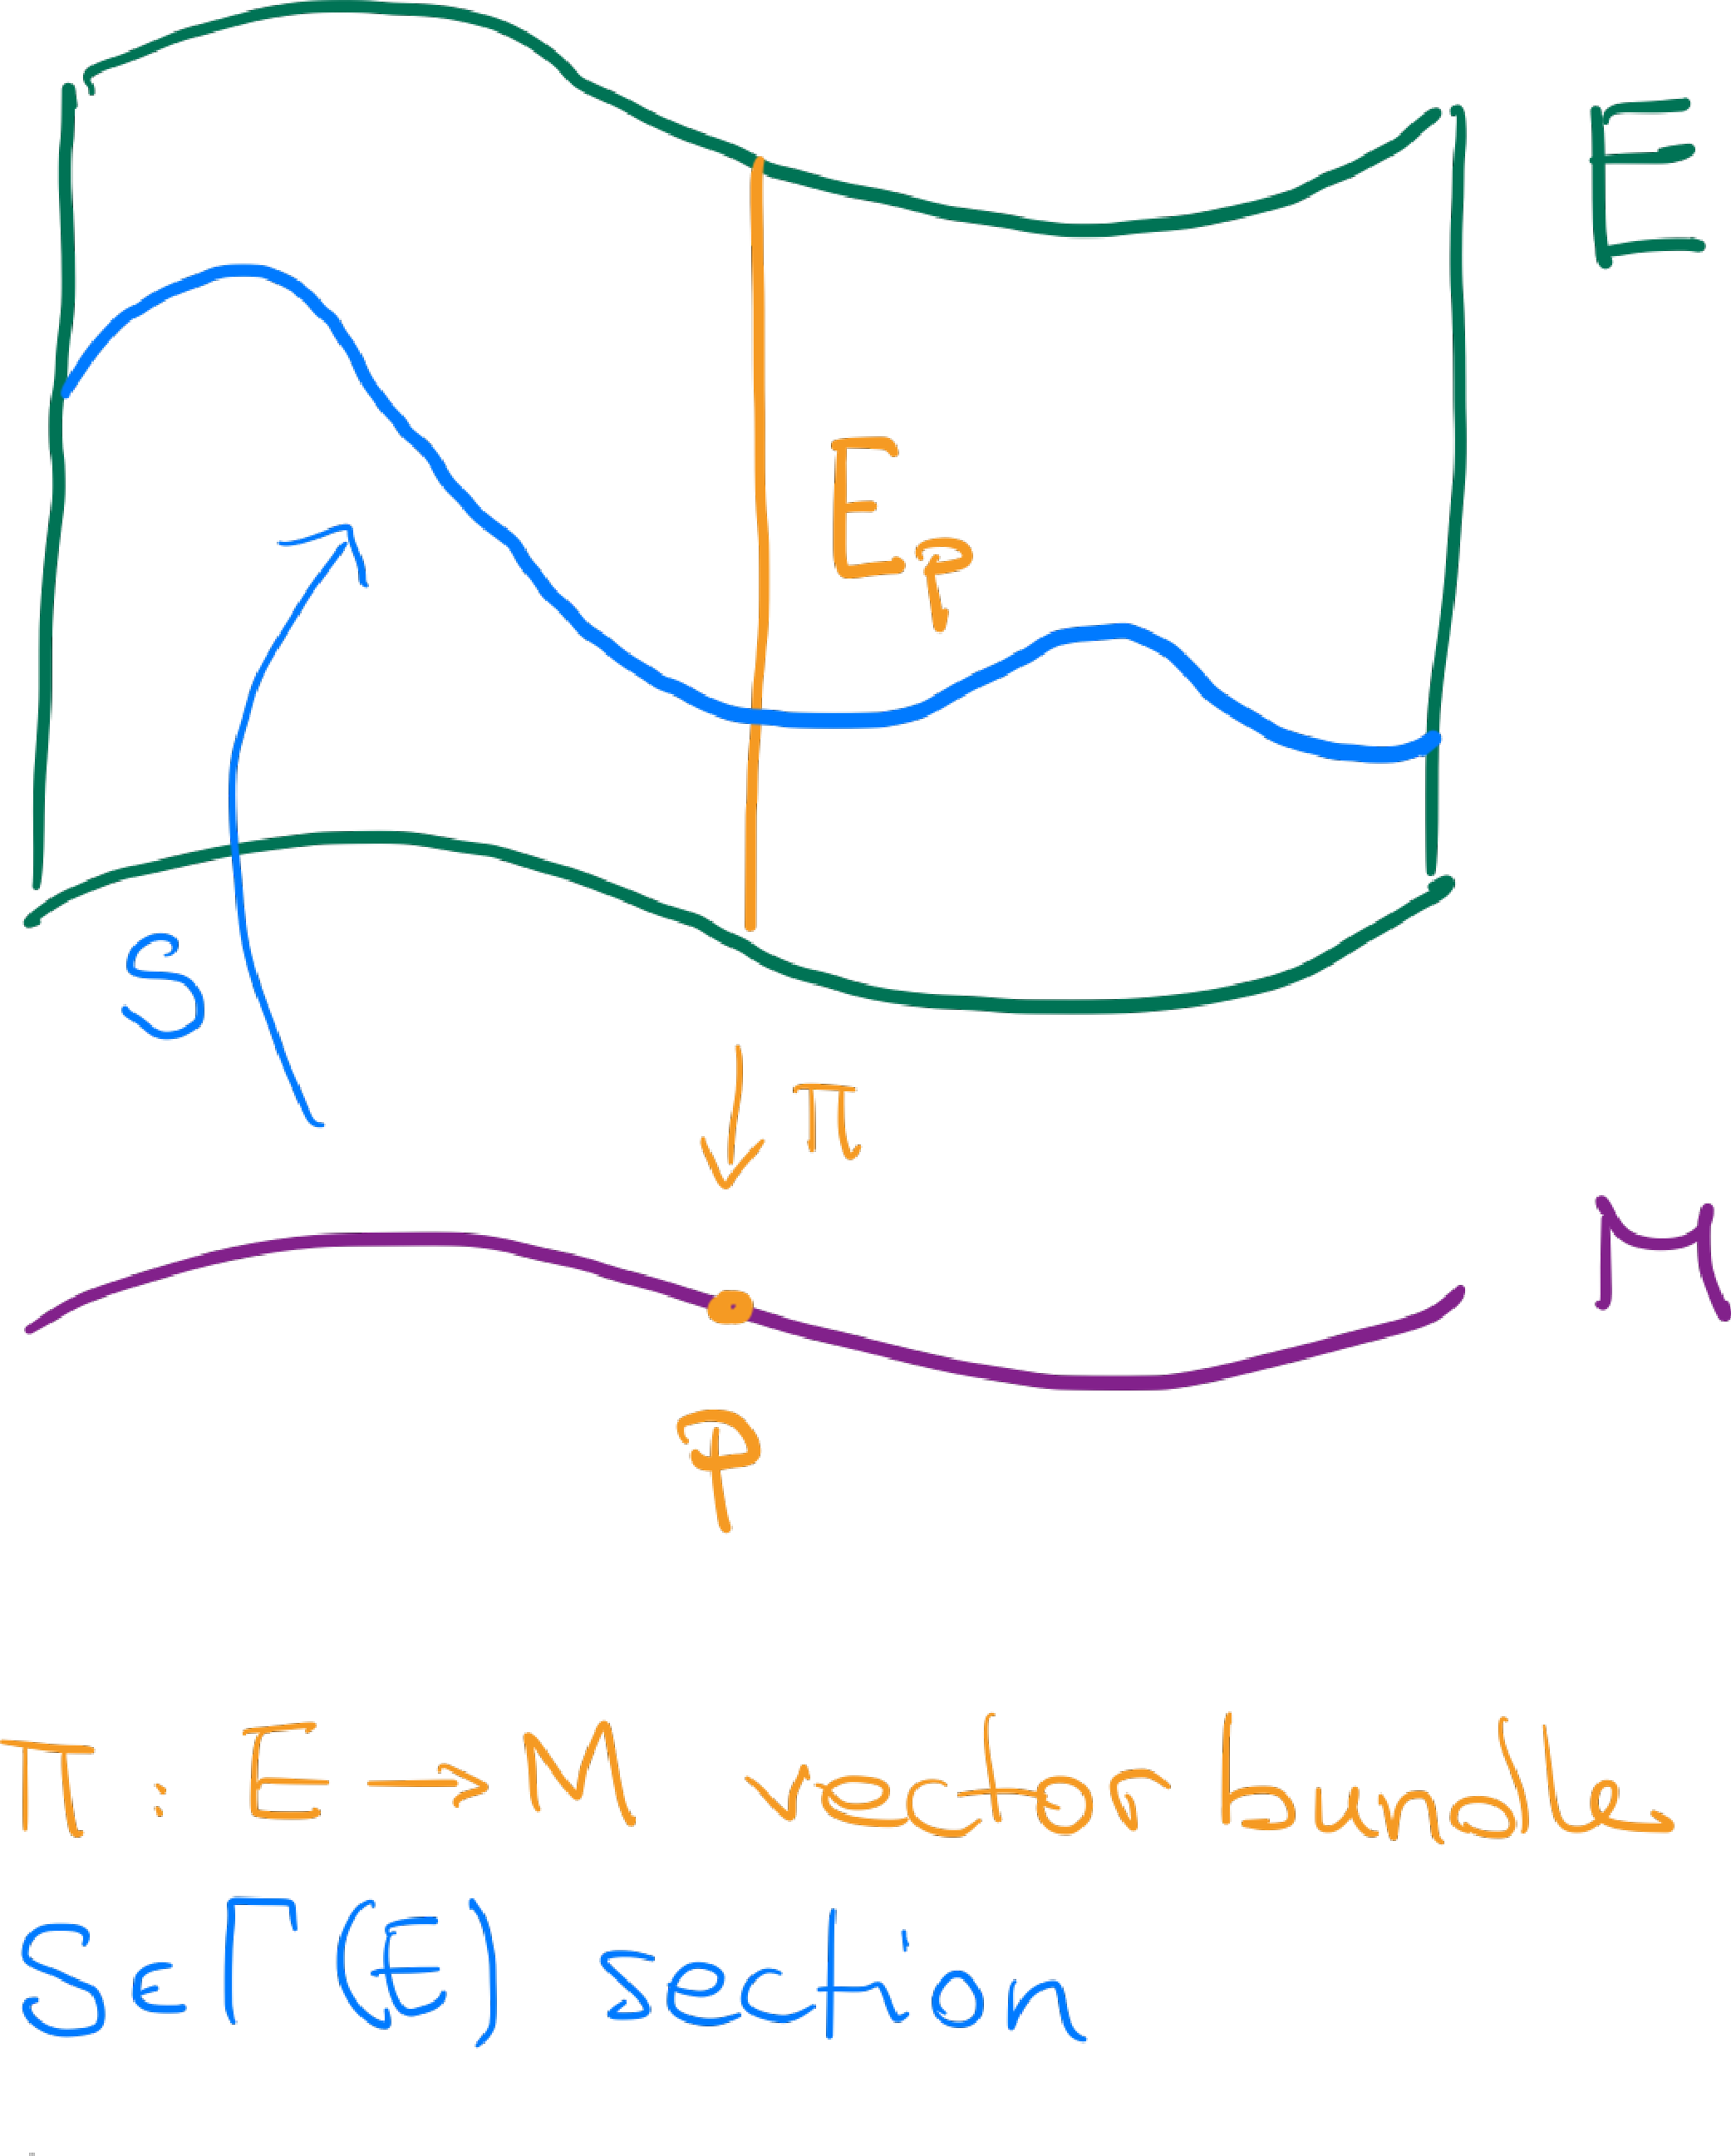
\includegraphics{2_7-bdl_section.pdf}
  \caption{A useful mnemonic to remember what is a section, is to imagine it as a cross-section of the bundle.}
\end{marginfigure}

\begin{definition}
  A \emph{section} of a vector bundle $\pi:E \to M$ is a smooth map $S:M \to E$ such that $\pi\circ S = \id_M$. We denote the set of all sections of $E$ by $\Gamma(E)$.

  If, in the definition, $M$ is replaced by $U\subset M$, the section is called \emph{local section}. The set of local sections on $U\subset M$ is denoted $\Gamma(E|_U)$.
\end{definition}

\begin{remark}
  A careful look at the definition shows that vector fields are sections of $TM$, indeed $\fX(M) \equiv \Gamma(TM)$.
  This is a useful way to start understanding the bundle terminology: in some sense, sections of vector bundles are a generalisation of vector fields.
\end{remark}

\begin{example}
If $E = M\times \R^r$, $M\subset\R^n$, then for any smooth map $F: M\to\R^r$ we have a section $S\in\Gamma(E)$ defined by $S(p) = (p, F(p))$. This is a classical euclidean vector field: a map that associates vectors to points (see Figure~\ref{fig:vectorfield-rn}).
  Notice, in particular, that functions $f\in C^\infty(M)$ are sections of the trivial bundle $M\times\R$.
\end{example}

One can sometimes distinguish non--isomorphic bundles by looking at the complement of their zero section: since any vector bundle isomorphism $h:E_1\to E_2$ must map the zero section of $E_1$ onto the zero section of $E_2$, the complements of the zero sections in $E_1$ and $E_2$ must be homeomorphic.

\begin{marginfigure}
    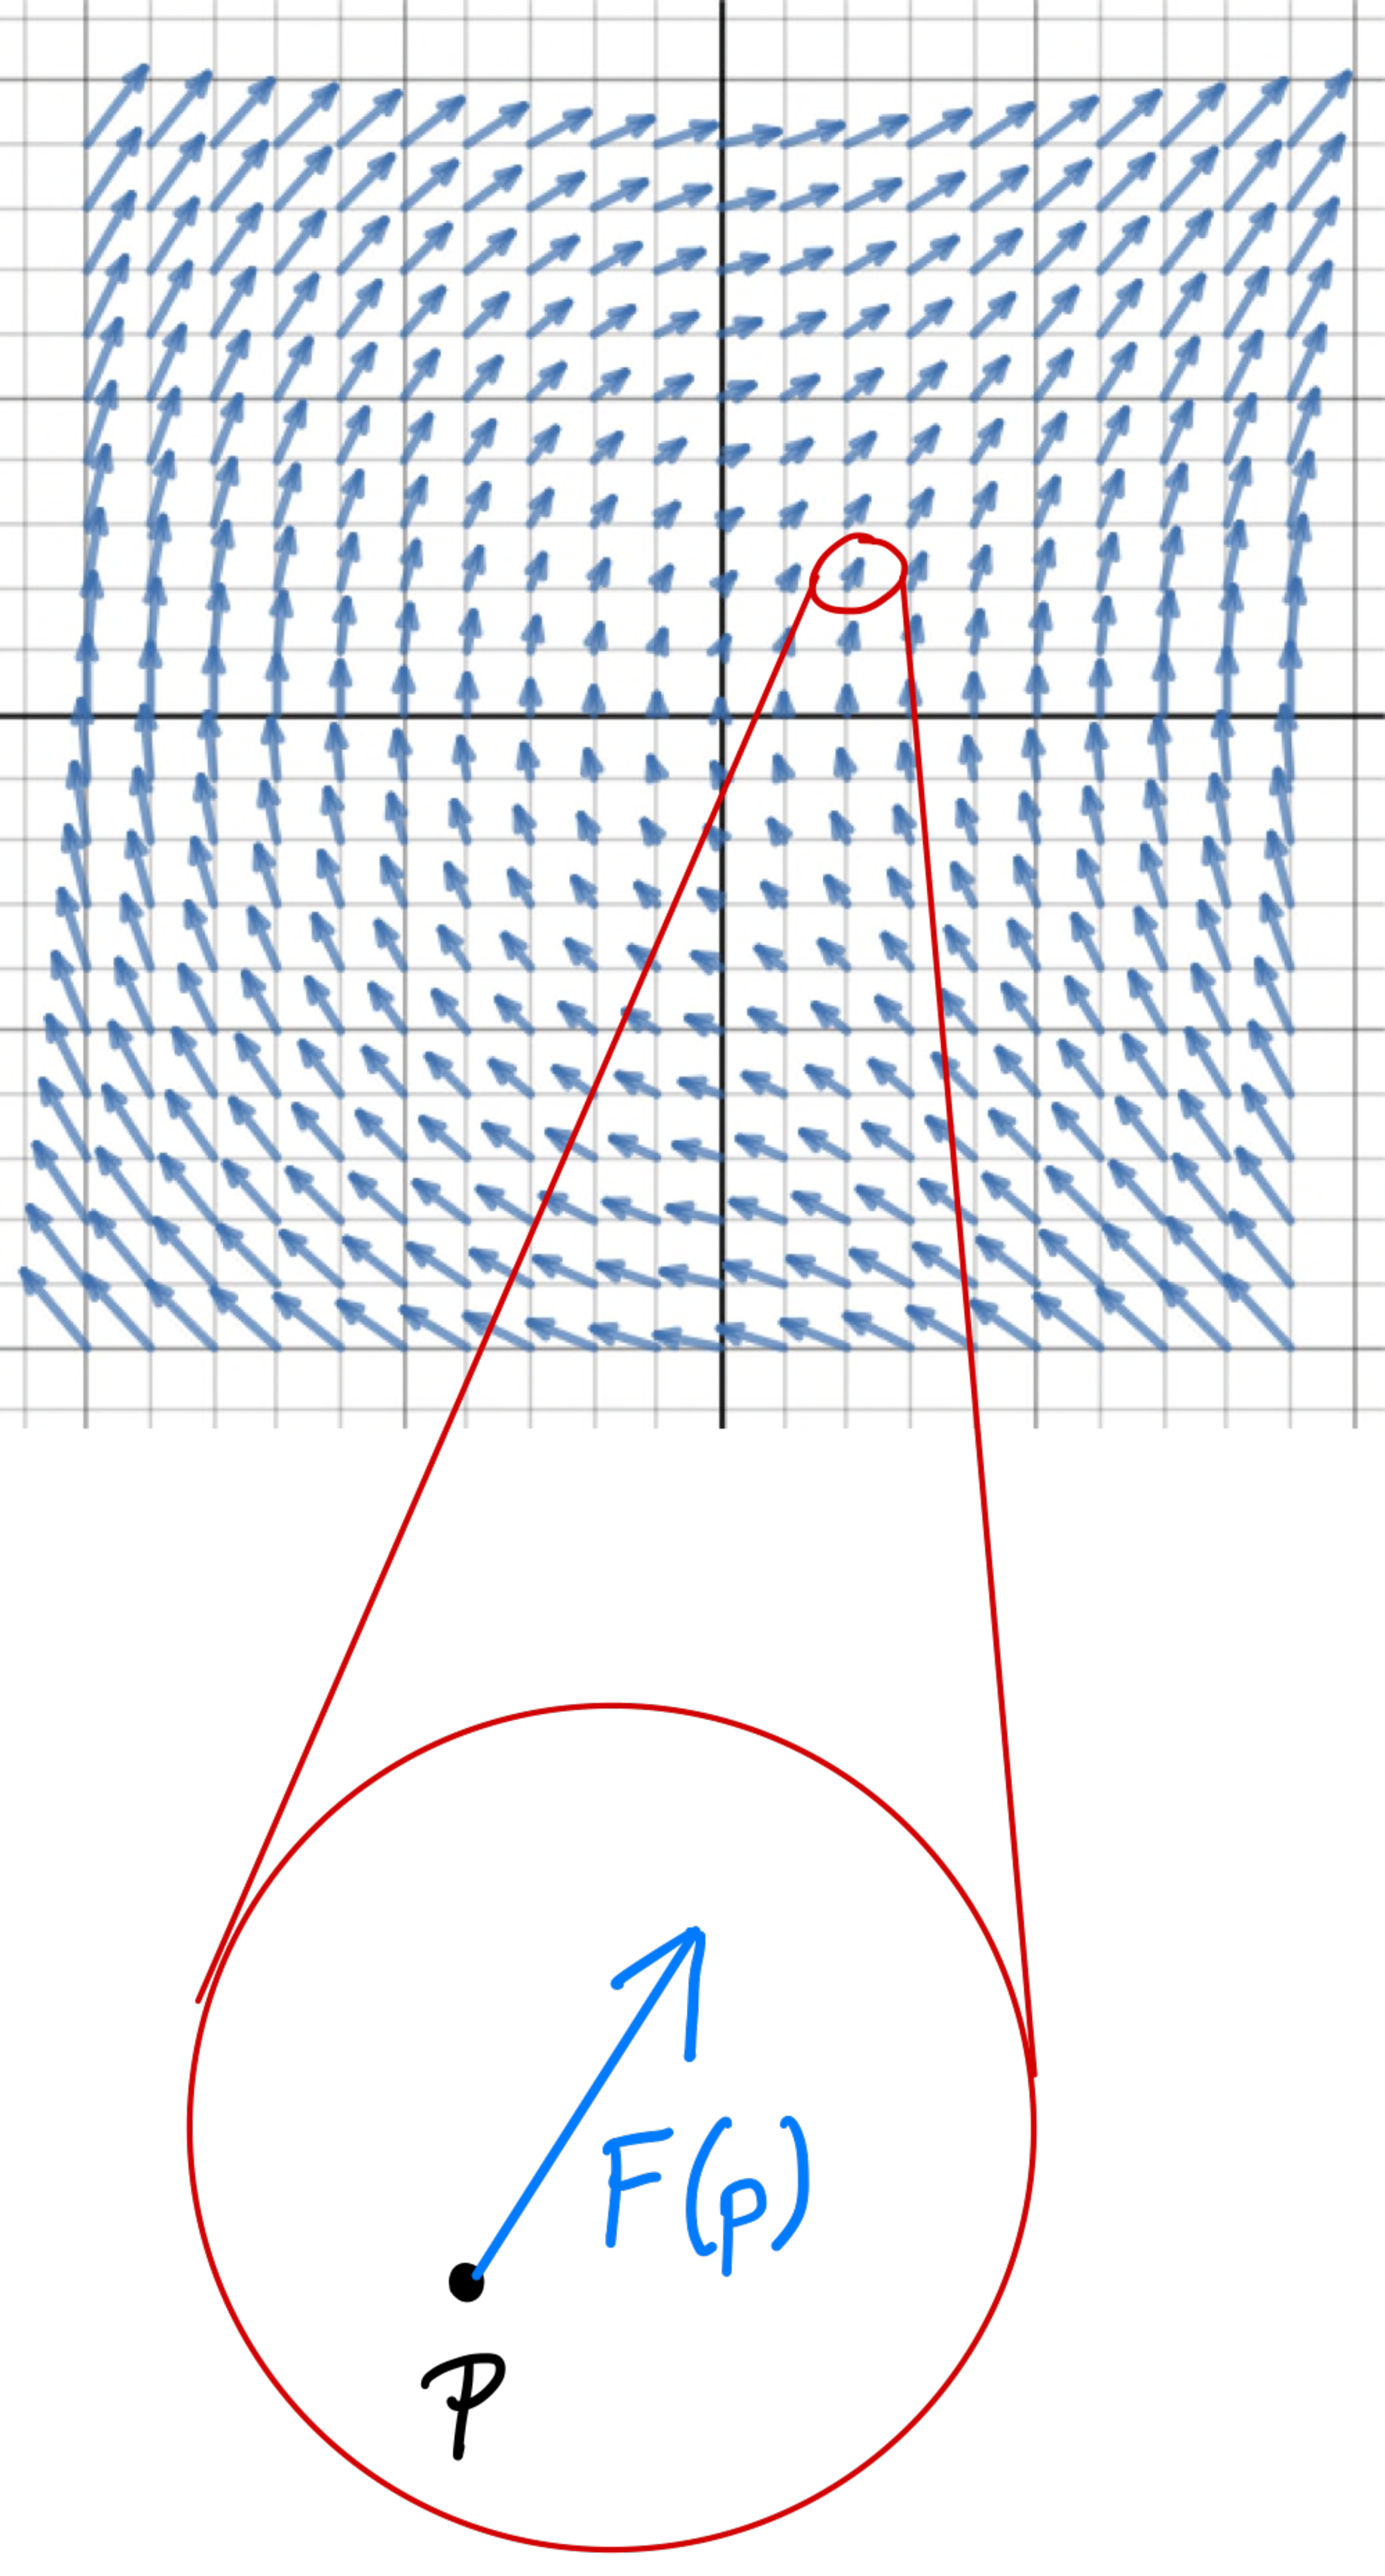
\includegraphics{2_9-vfield.pdf}
    \caption{A vector field ``attaches'' vectors to points.}%
    \label{fig:vectorfield-rn}
\end{marginfigure}

If the bundles are differentiable manifolds, then the definition of isomorphism nicely generalizes: they are \emph{diffeomorphic} if fibres are mapped to fibres diffeomorphically.

Even though, as we have seen, \emph{locally} $TM$ is diffeomorphic to $M\times\R^n$, this is not true in general with one exception.
\begin{exercise}\label{ex:trivialisable}
  Let $M$ be a smooth $n$-manifold that can be covered by a single smooth chart.
  Show that $TM$ is diffeomorphic to $M\times\R^n$ (without applying Proposition~\ref{prop:trivialisable}).
\end{exercise}

\begin{definition}
  A \emph{local frame} of a bundle $\pi:E\to M$ of rank $r$ is a family of $r$ local sections $\{S_1, \ldots, S_r\}\subset\Gamma(E|_U)$ such that $\{S_1(p), \ldots, S_r(p)\}$ is a basis for $E_p$ for all $p\in U$.
  If $U=M$ then $\{S_1, \ldots, S_r\}$ is called \emph{global frame}.
  Sometimes, the sections $S_j$ are called \emph{basis sections}.
\end{definition}

\begin{example}
  A chart on a $n$-manifold $M$ with local coordinates $(x^i)$ yields a local frame $\left\{\frac{\partial}{\partial x^1}, \ldots, \frac{\partial}{\partial x^n}\right\}$ of the tangent bundle $TM$.
\end{example}

In the spirit of what we have seen about the previous example, we have the following proposition.

\begin{proposition}
  Let $\pi:E \to M$ be a smooth vector bundle and $X:M\to E$ a section.
  If $\{S_i\}$ is a smooth local frame for $E$ over an open subset $U\subseteq M$, then $X$ is smooth on $U$ if and only if its component functions with respect to $\{S_i\}$ are smooth.
\end{proposition}
\begin{proof}
  Let $\varphi:\pi^{-1}(U) \to U\times\R^k$ be the local trivialization associated with the local frame $\{S_i\}$.
  Since $\varphi$ is a diffeomorphism, $X$ is smooth on $U$ if and only if $\varphi\circ X$ is smooth on $U$.
  If $\{X^i\}$ denotes the component function of $X$ with respect to $S_i$, then $\varphi\circ X (p) = (p, (X^1(p), \ldots, X^k(p)))$, so $\varphi\circ X$ is smooth if and only if the component functions $\{X^i\}$ are smooth.
\end{proof}

That is, given a local frame $\{S_1, \ldots, S_r\}\subset\Gamma(E|_U)$ of a vector bundle $\pi: E \to M$ we can express any section $X\in\Gamma(E)$ as a linear combination of elements of the frame:
\begin{equation}
  X = X^i S_i \quad\mbox{on }U,
\end{equation}
where $X^i\in C^\infty(U)$, $i=1,\ldots,r$.
Which was to be expected: after all, for each $p\in U\subset M$, the local frame is a basis for $E_p$.

\begin{proposition}\label{prop:trivialisable}
  A vector bundle $\pi: E\to M$ is trivialisable if and only if it admits a global frame.
\end{proposition}
\begin{proof}
  Let $\varphi: E \to M\times\R^r$ be a global trivialisation and $\{e_1, \ldots, e_r\}$ the canonical basis for $\R^r$.
  For $q\in M\times\R^r$, $\{S_1(q), \ldots, S_r(q)\} := \left\{\varphi^{-1}\big|_q(e_1), \ldots, \varphi^{-1}\big|_q(e_r) \right\}$ is a global frame for $E$ (why?).

  Conversely, let $\{S_1, \ldots, S_r\}$ be a global frame for $E$. Then
  \begin{equation}
    \varphi: E \to M\times\R^r, \quad
    \left(p, v^i S_i(p)\right) \mapsto \left(p, (v^1, \ldots, v^r)\right),
  \end{equation}
  is a global trivialisation for $E$.
\end{proof}

\begin{example}
  The cylinder $E = \bS^1\times\R$ is a trivialisable vector bundle with $\pi:E\to \bS^1$.
  Incidentally, the cylinder is isomorphic to $T\bS^1$ (why?).
\end{example}

\newthought{Of course, we can also define subbundles}.
\begin{definition}
  Let $\pi:E \to M$ be a rank-$r$ vector bundle and $F\subset E$ a submanifold.
  If for all $p\in M$, the intersection $F_p := F\cap E_p$ is a $k$-dimensional subspace of the vector space $E_p$ and $\pi|_F : F \to M$ defines a rank-$k$ vector bundle, then $\pi|_F: F \to M$ is called a \emph{subbundle} of $E$.
\end{definition}
\begin{marginfigure}
  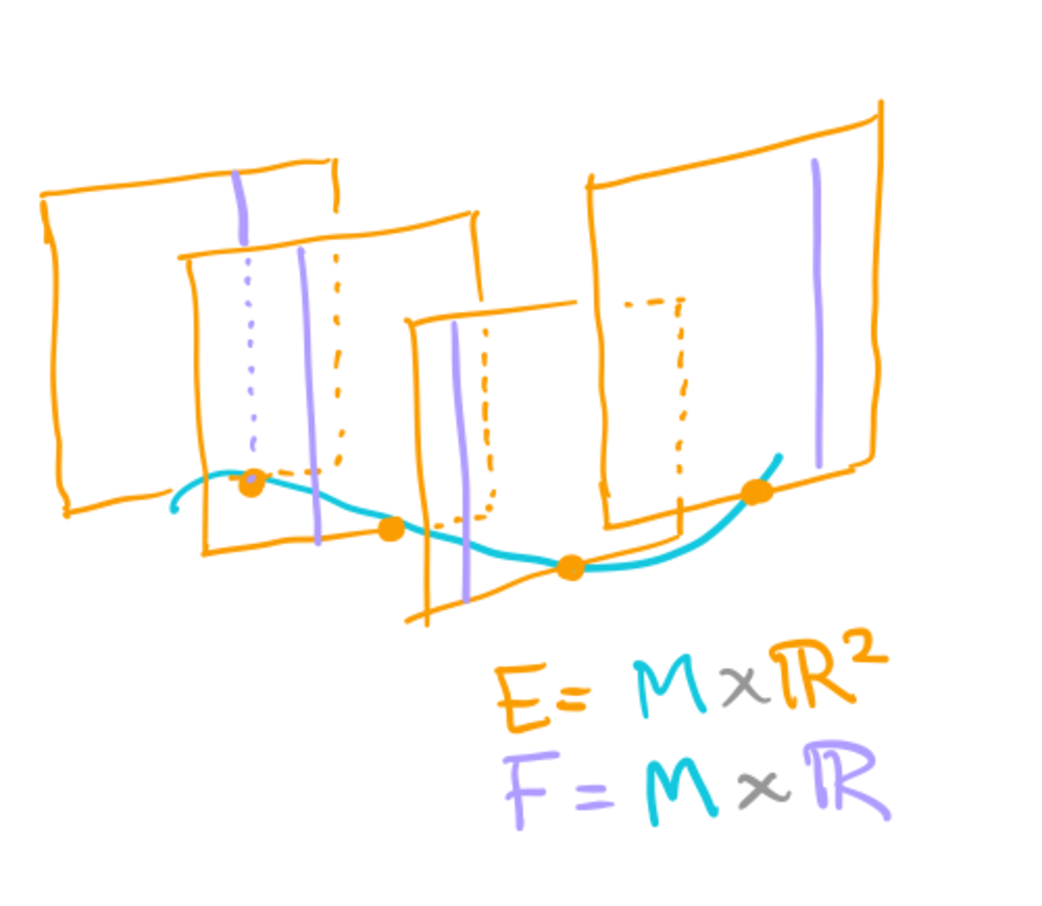
\includegraphics{images/2.10-subbundle.pdf}
\end{marginfigure}

\begin{exercise}
  Let $M$ be a smooth $m$-manifold and $N$ a smooth $n$-manifold.
  Let $F:M\to N$ be an embedding and denote $\widetilde M = F(M)\subset N$.
  \begin{enumerate}
    \item Show that the tangent bundle of $M$ in $N$, given by $T\widetilde M := dF(TM) \subset TN\big|_{\widetilde M}$, is a subbundle of $TN\big|_{\widetilde M}$ by providing explicit local trivialisations in terms of the charts $(U, \varphi)$ for $M$.
    \item Assume that there exist a smooth function $\Phi:N\to\R^{n-m}$ such that $\widetilde M := \{p\in N \mid \Phi(p) = 0\}$ and $d\Phi_p$ has full rank for all $p\in\widetilde M$. Prove that\footnote{Here $T\,N|_{\widetilde{M}}$ denotes the the tangent bundle of $N$ restricted to the base points in $\widetilde{M}$.}
          \begin{equation}
            T\widetilde{M} = \left\{(p,v)\in T\,N|_{\widetilde{M}} \mid v\in\ker(d\Phi_p)\right\}.
          \end{equation}
  \end{enumerate}
\end{exercise}

There are various useful generalization of vector bundles.
The \emph{fiber bundles} are bundles in which $\R$ is replaced by a more general manifold and are rather pervasive in mathematics and physics.
A special class of fiber bundles, the \emph{principal bundles}, have this manifold to be also a group with a well-defined action on the bundle.
Even if we will not discuss these examples in the notes, we will take a brief detour to discuss group actions, Lie groups and Lie algebras in the next chapter.
